\section{Introduction}\label{sec:intro}
\begin{comment}
In data mining, machine learning, and information retrieval, there is often a need to find data points in a dataset that are most similar or closely related to a given reference data point. This requirement gives rise to a fundamental operation known as the $k$ nearest neighbor (kNN) search.
%
The concept of the k-Nearest Neighbor Join (kNN join) operation \cite{bohm2004k}, extends the principles of kNN search.
% The concept of the $k$-nearest neighbor join (kNN join) operation~\cite{bohm2004k} was introduced after which extends kNN search.
%
Specifically, given two datasets, the query set $U$ and the answer set $I$, kNN join aims to identify for each data points in $U$, their kNN in $I$.
%
This approach, which involves a one-time computation of the kNN of \emph{all} data objects, has garnered considerable attention in the literature~\cite{bohm2004k,xia2004gorder,yu2007efficient, yu2010high, wang2010efficient, zhang2012efficient, lu2012efficient, yang2014continuous, zhao2017k,  amagata2019dynamic, shahvarani2021distributed, ukey2022efficient, ukey2023efficient} due to its efficiency compared to traditional single-query-based approaches.
%
Applications of kNN join includes classification~\cite{dasarathy1991nearest,zhang2017efficient}, clustering~\cite{hartigan1979algorithm, kanungo2002efficient}, recommendation system~\cite{hu2021efficient}, outlier detection ~\cite{ghoting2008fast, ning2018parameter}, etc.

In recent years, the emergence of big data applications, such as social networks, the Internet of Things (IoT), e-commerce platforms, and video streaming services, has posed new challenges for the kNN join problem. Data generated in such applications are typically characterised by their large volume, high dynamics, and high-dimensional nature.
%
For example, approximately $350,000$ tweets are sent per minute on Twitter as of 2020 \cite{tweets2010twitter}.
%
In popular social applications like Twitter, YouTube, Netflix, Instagram, and others, users (queries) and content (answers) are often represented as feature vectors in a high-dimensional space. The kNN join approach is commonly employed to return the k-nearest contents for each query based on their interests.
%
Similarly, E-commerce recommendation systems use kNN join to suggest products to consumers, thereby increasing the likelihood of purchases. The increasing demand for efficient kNN join techniques tailored to highly dynamic high-dimensional data is driven by the need to harness the full potential of newly generated data in these applications and provide fresh and timely recommendations.


In this paper, our focus is on dynamic kNN join over high-dimensional data, specifically the computation of \emph{exact} results for kNN join.
%
The demand for exact solutions in dynamic high-dimensional kNN join is highlighted by the phenomenon that in high-dimensional spaces distances between nearest and farthest points from query points become almost equal \cite{kouiroukidis2011effects}. Therefore, it is difficult for approximate methods to discriminate them.
%
Moreover, precision can also be crucial in many modern high-dimensional applications where data points may closely reside \cite{kassner2020bert, gupta2021retronlu, bonetta2021retrieval, han2023comprehensive, pan2023survey}.
\end{comment}

\begin{comment}
The $k$-nearest neighbors join (kNNj) is a fundamental operation in data science that formalizes the task of identifying, for each object in a query dataset $U$, its $k$ nearest neighbors from a reference dataset $I$. 
Unlike single-point neighbor search (kNN search), which focuses on the proximity relation of an individual query object, kNN join comprehensively establishes the neighborhood mapping between two datasets. 
This global perspective is crucial for applications that require exhaustive similarity coverage, a common demand across data-intensive industries. 

The importance of kNN join spans a wide spectrum of domains. 
In e-commerce and recommender systems, a prevalent strategy is to represent both users and items as vectors and to perform a kNN join between the corresponding user and item sets to discover potential matches or recommendations~\cite{hu2021efficient, yang2014continuous, ahuja2019movie}. 
In healthcare and biomedicine, kNN join supports disease prediction and diagnosis by analyzing relationships between preoperative risk factors and disease outcomes, as well as by enabling genomic profile matching~\cite{bhatti2021predictive, deekshatulu2013classification, khateeb2017efficient, tayeb2017toward}. 
Within vector database systems, it has emerged as a core query primitive of modern AI infrastructure, facilitating large-scale search and join operations over billions of high-dimensional vectors~\cite{pan2024vector, pan2024survey}. 
Beyond these examples, kNN join underpins a variety of machine learning tasks such as classification~\cite{bijalwan2014knn, deng2016efficient, dasarathy1991nearest, zhang2017efficient}, clustering~\cite{yang2016fault, shi2018adaptive, hartigan1979algorithm, kanungo2002efficient}, regression~\cite{kohli2020sales}, predictive modeling~\cite{jawthari2021predicting, baashar2021predicting}, and anomaly detection~\cite{li2007network, tian2014anomaly, wang2020log}. 
It also plays an essential role in fraud detection, by identifying transactions whose feature vectors are close to those of known fraudulent cases~\cite{al2021financial, li2023artificial, singhai2023novel, aldosari2024garra}, as well as in spatial data analysis~\cite{bohm2004k, xia2004gorder, yu2007efficient}, outlier detection~\cite{ghoting2008fast, ning2018parameter}, and broader KDD tasks~\cite{bohm2004k}. 
\end{comment}


\begin{comment}
finance:
In financial analytics, data points such as transactions, market events, and stock patterns are represented as high-dimensional feature vectors that evolve continuously over time. 
Because decision errors in these domains can incur substantial financial or regulatory consequences, 
systems require exact similarity evaluation rather than approximate search to ensure analytical reliability. 
To maintain consistent and precise risk assessment, the relationships between newly arriving data and their nearest historical counterparts must be preserved as an up-to-date adjacency network. 
This dynamically maintained similarity structure supports accurate fraud detection, stock pattern analysis, and market risk modeling, 
where new labeled cases or market conditions may instantly alter neighborhood relationships. 
Hence, the ability to maintain an exact kNN join under fully dynamic updates becomes essential for sustaining correctness in high-stakes financial decision making.

Healthcare:
In biomedical analytics, patient records and genetic profiles are represented as high-dimensional feature vectors derived from clinical indicators, imaging data, or genomic expressions. 
New patient samples are continuously collected, while medical case repositories and genomic reference databases are frequently updated as new studies and annotations become available. 
Maintaining an exact kNN join between the evolving patient and reference datasets is crucial for accurate similarity-based diagnosis, cohort identification, and genetic variant interpretation. 
By preserving an up-to-date neighborhood structure, clinicians and analytical systems can immediately reassess patient similarity relationships when new reference samples are introduced or outdated records are revised, 
ensuring diagnostic precision and consistency in a constantly evolving medical data environment.


网络安全：
In cybersecurity analytics, streams of system logs and network activities are continuously represented as high-dimensional behavioral vectors that describe protocol usage, temporal patterns, and host interactions.  
New activities are recorded every moment, while threat-signature repositories are constantly revised as confirmed attack traces are reported by external security services.  
Rather than labeling each event once and discarding it, detection systems maintain an evolving similarity network in which each activity remains linked to its closest historical counterparts.  
This persistent neighborhood structure allows risk scores to be updated whenever new malicious patterns are inserted or obsolete signatures are removed, ensuring precise and consistent intrusion recognition in an environment where both data and threat knowledge evolve.

物联网：
In industrial IoT systems, distributed sensors and controllers continuously emit high-dimensional feature vectors representing physical states, product quality, and environmental conditions.  
Maintaining an exact neighborhood graph over these evolving data streams is essential for real-time fault detection and predictive control, where each update may introduce new operational states or labeled fault cases.  
Recent studies have demonstrated the effectiveness of kNN-based classification and anomaly detection in industrial settings~\cite{wei2016multisensor,lei2023bearing},  
and further explored secure and distributed realizations of kNN analytics for large-scale IIoT infrastructures~\cite{yang2020seedknn}.  
However, existing approaches largely treat the data repository as static and perform one-shot queries, lacking the capability to dynamically maintain precise neighborhood relationships as both sensor readings and labeled references evolve over time.  
This motivates the need for a fully dynamic, exact kNN join framework capable of sustaining accurate and efficient proximity computations under continuous multi-source updates.

%%科学仿真
In scientific computing and engineering simulations, both experimental observations and simulated results are represented as high-dimensional feature vectors that capture complex physical or chemical behaviors.  
As new experiments are conducted and simulation parameters are refined, both datasets evolve continuously, requiring their similarity relationships to be updated for accurate model validation and result correlation.  
Maintaining an exact kNN join between the evolving experimental and simulated data enables researchers to identify matching patterns, verify model fidelity, and trace parameter sensitivities over time.  
This persistent and precise neighborhood structure supports reproducible analysis and cross-validation across successive simulation cycles, where approximation errors or stale neighbor mappings could lead to incorrect scientific conclusions.


\end{comment}




\begin{comment}
The k-Nearest Neighbors join (kNNj) is a fundamental operation in data science that formalizes the task of retrieving the $k$ nearest neighbors from a reference dataset $I$ for every point within a given query dataset $U$. Covering all the data points in $U$ rather than only exploring the neighbor relation with $I$ of an individual point, kNN join establishes a comprehensive mapping of proximity relationships between two datasets. This global perspective is of significant importance in the big data industry, particularly for application domains that necessitate exhaustive coverage for all potential similarity searches. kNN join demonstrates broad utility across diverse domains. In e-commerce platforms and recommender systems, a common approach is to project both users and items in a vector space and perform a kNN join between the user-vector set and the item-vector set to discover potential targets \cite{hu2021efficient, yang2014continuous, ahuja2019movie}. In healthcare and biomedicine, it supports disease prediction and diagnosis by analyzing connections between preoperative risk variables and diseases, as well as genomic profile matching \cite{bhatti2021predictive, deekshatulu2013classification, khateeb2017efficient, tayeb2017toward}. In vector databases, kNN join now serves as the core query primitive of modern AI infrastructure, enabling efficient search and join over billions of high-dimensional vectors \cite{pan2024vector, pan2024survey}. Beyond these, kNN join is applied in machine learning tasks such as classification \cite{bijalwan2014knn, deng2016efficient,dasarathy1991nearest,zhang2017efficient}, clustering \cite{yang2016fault, shi2018adaptive, hartigan1979algorithm, kanungo2002efficient}, regression \cite{kohli2020sales}, predictive systems \cite{jawthari2021predicting, baashar2021predicting}, and anomaly detection \cite{li2007network, tian2014anomaly, wang2020log}. It also supports fraud detection by surfacing transactions whose corresponding vectors are close to historical fraud cases \cite{al2021financial, li2023artificial, singhai2023novel, aldosari2024garra}, as well as spatial data analysis \cite{bohm2004k,xia2004gorder,yu2007efficient}, outlier detection \cite{ghoting2008fast, ning2018parameter}, and broader KDD tasks \cite{bohm2004k}. Modern applications proposes a new demand for kNN join algorithms with high dimensionality and data dynamism. In e-commerce and media streaming, firms like Amazon and Netflix utilize high-dimensional vectors, which imposes the curse of dimensionality to the kNN operations. Simultaneously, the demand for dynamic adaptivity is driven by sectors with constantly changing data, including social media platforms like TikTok and Twitter (which sees over 300,000 tweets per minute \cite{tweets2010twitter}), as well as real-time financial services.
\end{comment}

\begin{comment}
Modern data-intensive applications now demand kNN join algorithms that can efficiently operate under both high dimensionality and continuous data evolution. 
In large-scale recommendation and media platforms, user and item embeddings are frequently updated or regenerated, making both the query and reference datasets highly dynamic. 
Similarly, real-time analytics and vector databases must accommodate incessant insertions and deletions on both sides of the join. 
These fully dynamic settings have become increasingly common in modern AI-driven infrastructures, yet existing research has almost exclusively focused on \emph{partially dynamic} scenarios where only one dataset changes while the other remains static.

At the same time, the rapid increase in feature dimensionality—often reaching hundreds or even thousands of dimensions in industrial embeddings—has made the cost of distance computations a dominant performance bottleneck. 
Previous studies typically rely on coarse-grained or heuristic rules to select the reduced dimensionality for pruning, overlooking the quantitative trade-off between projection dimension and computational cost.
\end{comment}



The $k$-nearest neighbors join (kNNj) is a fundamental operation in data science that formalizes the task of identifying, for each object in a query dataset $U$, its $k$ nearest neighbors from a reference dataset $I$. Unlike single-point neighbor search (kNN search), which focuses on the proximity relation of an individual query object, kNN join comprehensively establishes the neighborhood mapping between two datasets. This global perspective is crucial for applications that require exhaustive similarity coverage, a common demand across data-intensive industries. The importance of kNN join spans a wide spectrum of domains. In e-commerce and recommender systems, a prevalent strategy is to represent both users and items as vectors and to perform a kNN join between the corresponding user and item sets to discover potential matches or recommendations~\cite{hu2021efficient, yang2014continuous, ahuja2019movie}. In healthcare and biomedicine, kNN join supports disease prediction and diagnosis by analyzing relationships between preoperative risk factors and disease outcomes, as well as by enabling genomic profile matching~\cite{bhatti2021predictive, deekshatulu2013classification, khateeb2017efficient, tayeb2017toward}. Within vector database systems, it has emerged as a core query primitive of modern AI infrastructure, facilitating large-scale search and join operations over billions of high-dimensional vectors~\cite{pan2024vector, pan2024survey}. Beyond these examples, kNN join underpins a variety of machine learning tasks such as classification~\cite{bijalwan2014knn, deng2016efficient, dasarathy1991nearest, zhang2017efficient}, clustering~\cite{yang2016fault, shi2018adaptive, hartigan1979algorithm, kanungo2002efficient}, regression~\cite{kohli2020sales}, predictive modeling~\cite{jawthari2021predicting, baashar2021predicting}, and anomaly detection~\cite{li2007network, tian2014anomaly, wang2020log}. It also plays an essential role in fraud detection, by identifying transactions whose feature vectors are close to those of known fraudulent cases~\cite{al2021financial, li2023artificial, singhai2023novel, aldosari2024garra}, as well as in spatial data analysis~\cite{bohm2004k, xia2004gorder, yu2007efficient}, outlier detection~\cite{ghoting2008fast, ning2018parameter}, and broader KDD tasks~\cite{bohm2004k}.

\begin{comment}
Today, the paradigm for data joins is shifting from the static or \emph{partially}-dynamic model to \emph{fully}-dynamic ecosystems, where both query and reference sets are concurrently updated. For example, clinical genomics sees patient data and reference panels evolve continuously \cite{mukherjee2023iot, reddy2022novel, bharadwaj2021review}, and financial analytics \cite{lin2021multidimensional, li2023artificial, gao2024machine} churns on real-time transaction streams. Despite this, most existing kNN (join) methods are designed for static collections or assume
one-sided updates, leaving the fully dynamic setting underexplored
and its systems implications insufficiently addressed.
\end{comment}

\noindent \textbf{FULLY-DYNAMIC HIGH DIMENSIONAL KNNJ.} The paradigm for data joins is evolving to meet the dual challenges of increasing data dimensionality and the shift from static or partially-dynamic models to fully-dynamic ecosystems, where both query and reference sets are concurrently updated. This evolution is also pronounced in high-stakes, low-tolerance domains. In clinical genomics \cite{mukherjee2023iot, reddy2022novel, bharadwaj2021review}, for instance, high-dimensional patient data and genomic reference panels evolve continuously, while financial analytics churns on high-dimensional, real-time transaction streams \cite{lin2021multidimensional, li2023artificial, gao2024machine}. Such scenarios are therefore defined by both their fully-dynamic, high-dimensional nature and their stringent requirement for the precision of exact kNN joins. This confluence of requirements establishes the problem of performing exact, high-dimensional kNN joins in fully-dynamic settings as a new and critical research frontier.

\noindent\textbf{APPLICATIONS.} The problems of High-dimensional and fully-dynamic kNN join underpin numerous critical applications across modern data-intensive systems.

In financial analytics \cite{rao2024hybrid, lin2021multidimensional, pillai2024financial, li2023artificial, gao2024machine}, transactions and market patterns are represented as high-dimensional feature vectors. The query set comprises the continuous stream of new transactions, while the reference set is the constantly evolving database of historical, labeled cases (e.g., confirmed fraud). To ensure consistent and reliable outcomes in this high-stakes domain, analytical methods that provide verifiable precision are highly valued. An exact kNN join is well-suited to this need, offering a deterministic guarantee that every transaction is compared against the most up-to-date precedents for robust risk modeling and fraud detection.

In biomedical analytics \cite{reddy2022novel, mukherjee2023iot, al2025dynamic, bharadwaj2021review}, patient records and genetic profiles are represented as high-dimensional feature vectors. The query set is composed of newly collected patient samples, while the reference set includes constantly evolving medical case repositories and genomic databases. Given that diagnostic errors can lead to severe health consequences, this low-tolerance domain demands exceptional analytical precision. An exact kNN join meets this requirement by enabling immediate and precise reassessment of patient similarity against the latest reference data, which is crucial for accurate diagnosis and cohort identification.

In cybersecurity \cite{chen2017survey, singh2024network, qi2021detecting, xu2020combination}, network activities and system logs are modeled as high-dimensional behavioral vectors. The query set comprises the continuous stream of new events, while the reference set is the repository of threat signatures, which is constantly revised with new intelligence. The reliability of intrusion detection systems in this context benefits from the high-fidelity application of threat intelligence. An exact kNN join supports this objective by ensuring that every new event is deterministically compared against the most current threat knowledge base, providing a consistent and verifiable foundation for risk assessment.

In industrial IoT systems \cite{kumar2015hybrid, wei2016multisensor, wang2021weighted, yang2020secure,younes2021efficient}, sensor readings are represented as high-dimensional feature vectors describing machinery states. The query set consists of the continuous stream of these readings, while the reference set is the evolving library of labeled operational states, including known fault cases. To ensure operational safety and reliability, it is beneficial to maintain a verifiable link between real-time sensor readings and known operational states. An exact kNN join facilitates this by preserving precise neighborhood relationships as both sensor data and labeled references evolve over time.

In scientific computing \cite{giommi2023machine, kheddar2024image, shivahare2022survey}, both experimental observations and simulation results are captured as high-dimensional feature vectors. The query set is typically composed of new experimental observations as they are collected, while the reference set consists of an evolving repository of simulation results, which is updated as model parameters are refined across successive runs. The integrity and reproducibility of research in this domain often depend on the determinism and precision of the underlying analysis, as approximation errors could lead to incorrect scientific conclusions. An exact kNN join is therefore well-suited for this requirement, enabling researchers to accurately match experimental outcomes to their closest simulated counterparts, which is essential for model validation and result correlation.

\begin{comment}
At the same time, modern vectors routinely span hundreds to thousands of dimensions. Modeling both the distribution of data points in the ambient space and the relationship between projection dimensions and projected distances is mathematically nontrivial. As a result, prior work typically chooses the reduced dimensions heuristically, preventing pruning from achieving maximal efficiency.
\end{comment}



\begin{comment}
This paper introduces the \emph{fully dynamic kNN join} problem on high-dimensional data and presents a new solution framework, \emph{\dualtree}. 
Our approach employs a symmetric dual-index structure that jointly maintains an \hdrtree\ on the query set and a \deltatree\ on the reference set, enabling efficient bidirectional kNN and reverse kNN processing under continuous updates. 
Furthermore, we develop a theoretical cost model that explicitly characterizes the relationship between dimensionality and pruning efficiency, from which we derive the optimal projection dimension that maximizes computational efficiency.
\end{comment}

\begin{comment}
To close these gaps, we present \dualtree, a dual-indexing framework that realizes efficient kNN joins in fully dynamic, high-dimen\-sional settings. Beyond the architecture, we integrate a fine-grained pruning step driven by a mathematic model that evaluates the trade-off between projection dimensions and the computational cost, thereby maximizing the pruning efficiency.
\end{comment}

\begin{comment}
\stitle{Existing Solutions.}
%
The naive approach to computing exact kNN join employs a brute-force method, searching for proximity among all data points for each update. This approach leads to a substantial computational complexity, especially in high-dimensional spaces, and is impractical for real-world applications.
%
% index
% dimensionality reduction
While many existing works have focused on static datasets \cite{bohm2004k,xia2004gorder,yu2007efficient}, dynamic methods \cite{yu2010high, yang2014continuous, ukey2022efficient, ukey2023efficient,ukey2023knn} have been proposed in the past decade to speed up dynamic kNN join over high-dimensional data.
%
To improve efficiency, state-of-the-art solutions for dynamic kNN join over high-dimensional data typically adopt two techniques, namely \emph{indexing} and \emph{dimensionality reduction}.
%
Example indexing data structures include R-trees in \cite{guttman1984r, zhang2012efficient, prasad2015gpu}, \hdrtree in \cite{yang2014continuous,ukey2022efficient,ukey2023efficient,ukey2023knn}, and iDistance in \cite{yu2007efficient, yu2010high}.
%
These algorithms utilise the index to quickly identify potential $k$ nearest neighbors, rather than exhaustively comparing distances between the query point and every data point in the dataset to narrow down search space. 
%
When it comes to dimensionality reduction, one of the most commonly used techniques for exact kNN join is Principal Component Analysis (PCA) \cite{wold1987principal, chakrabarti2000local, abdi2010principal, vidal2016principal}.
%
PCA is employed to transform high-dimensional data into a lower-dimensional space while retaining useful information, resulting in faster and more cost-effective computations. 
%
Dimensionality reduction is essential to tackle the ``curse of dimensionality'' problem \cite{beyer1999nearest, kouiroukidis2011effects}, which arises with high-dimensional data.
\end{comment}

\begin{comment}
\noindent\textbf{EXISTING WORK.} A broad lineage of kNN join methods has been studied over the past two decades \cite{gao2023high, gu2018approximate, sun2014srs, zhao2023towards, andoni2008near, li2019approximate, cui2005exploring, bohm2004k, xia2004gorder, yu2007efficient, yu2001indexing, bohm2006efficiently, yu2010high, cui2003contorting}. Tn order to handle critical scenarios where very high precision is required, a series of representative exact systems including MuX \cite{bohm2004k}, Gorder \cite{xia2004gorder}, iJoin \cite{yu2007efficient}, iDistance \cite{yu2001indexing}, the grid-based streaming method of Böhm et al. \cite{bohm2006efficiently}, and kNNJoin$^{+}$ \cite{yu2010high} has been proposed. However, these systems either do not support dynamic updates on the sets involved or exhibit degraded effectiveness in high dimensional context. To move closer to practical requirements, \hdrtree \cite{yang2014continuous}, \deltatree \cite{cui2003contorting}, and various variants and improvements of these two structures \cite{ukey2022efficient, ukey2023efficient, ukey2024cluster} have also been proposed emerged to support dynamic kNN joins in high-dimensional spaces. However, their dynamism is partial: \hdrtree accelerates cases where only the reference set is updated, while \deltatree targets updates confined to the query set. Consequently, both fall short of addressing the fully- dynamic, high-dimensional regime in which \emph{both} sets evolve concurrently. Despite their difference, most of the exact kNN join systems mentioned above adopt an indexing plus dimensionality reduction paradigm to realize efficient and exact kNN join. And among their dimensionality reduction mechanisms, the projection dimensionalities are typically chosen heuristically; to our knowledge, no prior work provides a quantitative model that relates projection dimensionalities to computational cost for selecting an optimal pruning dimensionality.
\end{comment}

\noindent\textbf{EXISTING WORK.} A broad lineage of kNN join methods has been studied over the past two decades \cite{gao2023high, gu2018approximate, sun2014srs, zhao2023towards, andoni2008near, li2019approximate, cui2005exploring, bohm2004k, xia2004gorder, yu2007efficient, yu2001indexing, bohm2006efficiently, yu2010high, cui2003contorting}. While numerous exact systems have been proposed for high-precision applications \cite{bohm2004k, xia2004gorder, yu2007efficient, yu2001indexing, bohm2006efficiently, yu2010high, cui2003contorting, yang2014continuous, ukey2022efficient, ukey2023efficient, ukey2024cluster}, they are constrained by two fundamental limitations. First, they are ill-suited for the emerging fully-dynamic, high-dimensional regime. Second, although many adopt a dimensionality reduction and pruning paradigm to mitigate the heavy cost of full-dimensional distance calculations in high-dimensional space resulting from the curse of dimensionality \cite{altman2018curse}, the projection dimensionality for pruning is typically chosen heuristically. To our knowledge, no prior work provides a quantitative model that relates projection dimensionality to computational cost, thus preventing the selection of an optimal dimension that would maximize pruning efficiency.


\stitle{Motivation.}
%
Modern deployments increasingly require kNN joins to operate in fully dynamic environments, yet most existing designs remain static or partially dynamic and leave this regime underexplored. In parallel, most of the prior kNN join systems typically pair indexing with cluster-level pruning in heuristically chosen low-dimensional space, while (i) overlooking deeper, point-wise low-dimensional pruning and (ii) lacking a quantitative model that relates the projection dimensionality to computational cost; consequently, pruning cannot be driven to maximal efficiency.

\begin{comment}
\begin{enumerate} [leftmargin=*, wide, labelindent=0pt]
    \item \underline{\emph{Partial Support for Dynamic Data Updating.}}
    To the best of our knowledge, all existing solutions have focused on \emph{partial} dynamic kNN join scenarios \cite{ukey2023survey}, where updates typically occur in the answer set, overlooking the dynamic changes within the query set.
    %    
    However, it is common in real-world applications for both the query and the answer set to update simultaneously.
    %
    We refer to the problem of maintaining the results of kNN join when both the query and answer sets can update simultaneously and arbitrarily as \emph{fully} dynamic kNN join (\fdknnj).
    %
    We observe that no existing methods efficiently handle \fdknnj over high-dimensional data.

    \item \underline{\emph{Massive Distance Computation in High Dimensions.}}
    %
    Computing distances among high-dimensional data is a computationally intensive task in dynamic kNN join. Existing methods leverage dimensionality reduction, projecting data from high-dimensional space to a lower-dimensional one and eliminating unpromising candidates. This reduces the number of distance computations in the full dimension.
    %
    However, current pruning strategies \cite{yu2007efficient, yu2010high, yang2014continuous, ukey2022efficient, ukey2023efficient} are \textit{coarse-grained}, typically at the node/cluster level in the index tree structure. This coarse-grained and node-based pruning often leaves a significant number of unpromising candidates, leading to suboptimal results.
    %
    For instance, in on of the commonly used index, the \hdrtree, we observed that leaf nodes still contain over $90\%$ of unpromising data points in the NUS-WIDE \cite{chua2009nus} dataset during updates by applying a coarse-grained pruning.
    
\end{enumerate}
\end{comment}

\noindent (a)\underline{\emph{Partial Support for Dynamic Data Updating.}}
    Recent years have seen kNN-based machine-learning techniques move from niche utilities to widely deployed practice \cite{pan2023survey, li2023artificial, shivahare2022survey, ridwan2021applications, an2023comprehensive}. As industrial workloads have matured, data has become increasingly dynamic—updates are more frequent, more pervasive, and extend deeper into operational pipelines \cite{li2024tracking, immadisetty2025real, almeida2023time}. However, kNN join research has not kept pace: most methods still target static collections or one-sided updates, leaving fully dynamic operation underexplored. To close this gap, we introduce a dual-index design that enables efficient kNN joins across the full spectrum of dynamic workloads.

\noindent (b) \underline{\emph{Limitations in Pruning and Dimensionality Selection.}} Most prior kNN join systems reduce full-dimensional distance costs via cluster-level pruning in a low-dimensional space. However, this coarse granularity yields many false positives that are then handled in the full dimensions, with little or no point-wise low-dimensional pruning to further filter candidates. Moreover, the projection dimensionality is typically chosen heuristically, as modeling the probability distribution of the interpoint distance and the relation between the projection distance and the projection dimensionality is mathematically challenging—leaving the pruning potential underexploited. In response, we integrate a point-wise, fine-grained pruning stage into our dual-index design and develop a cost-aware model to select the projection dimensionality, driving pruning toward maximal efficiency.
    
    



\begin{comment}
\stitle{Applications.} 
%
\fdknnj can offer substantial benefits for a wide range of applications across diverse domains. We provide some examples as follows.

\begin{figure}[t]
    \centering
    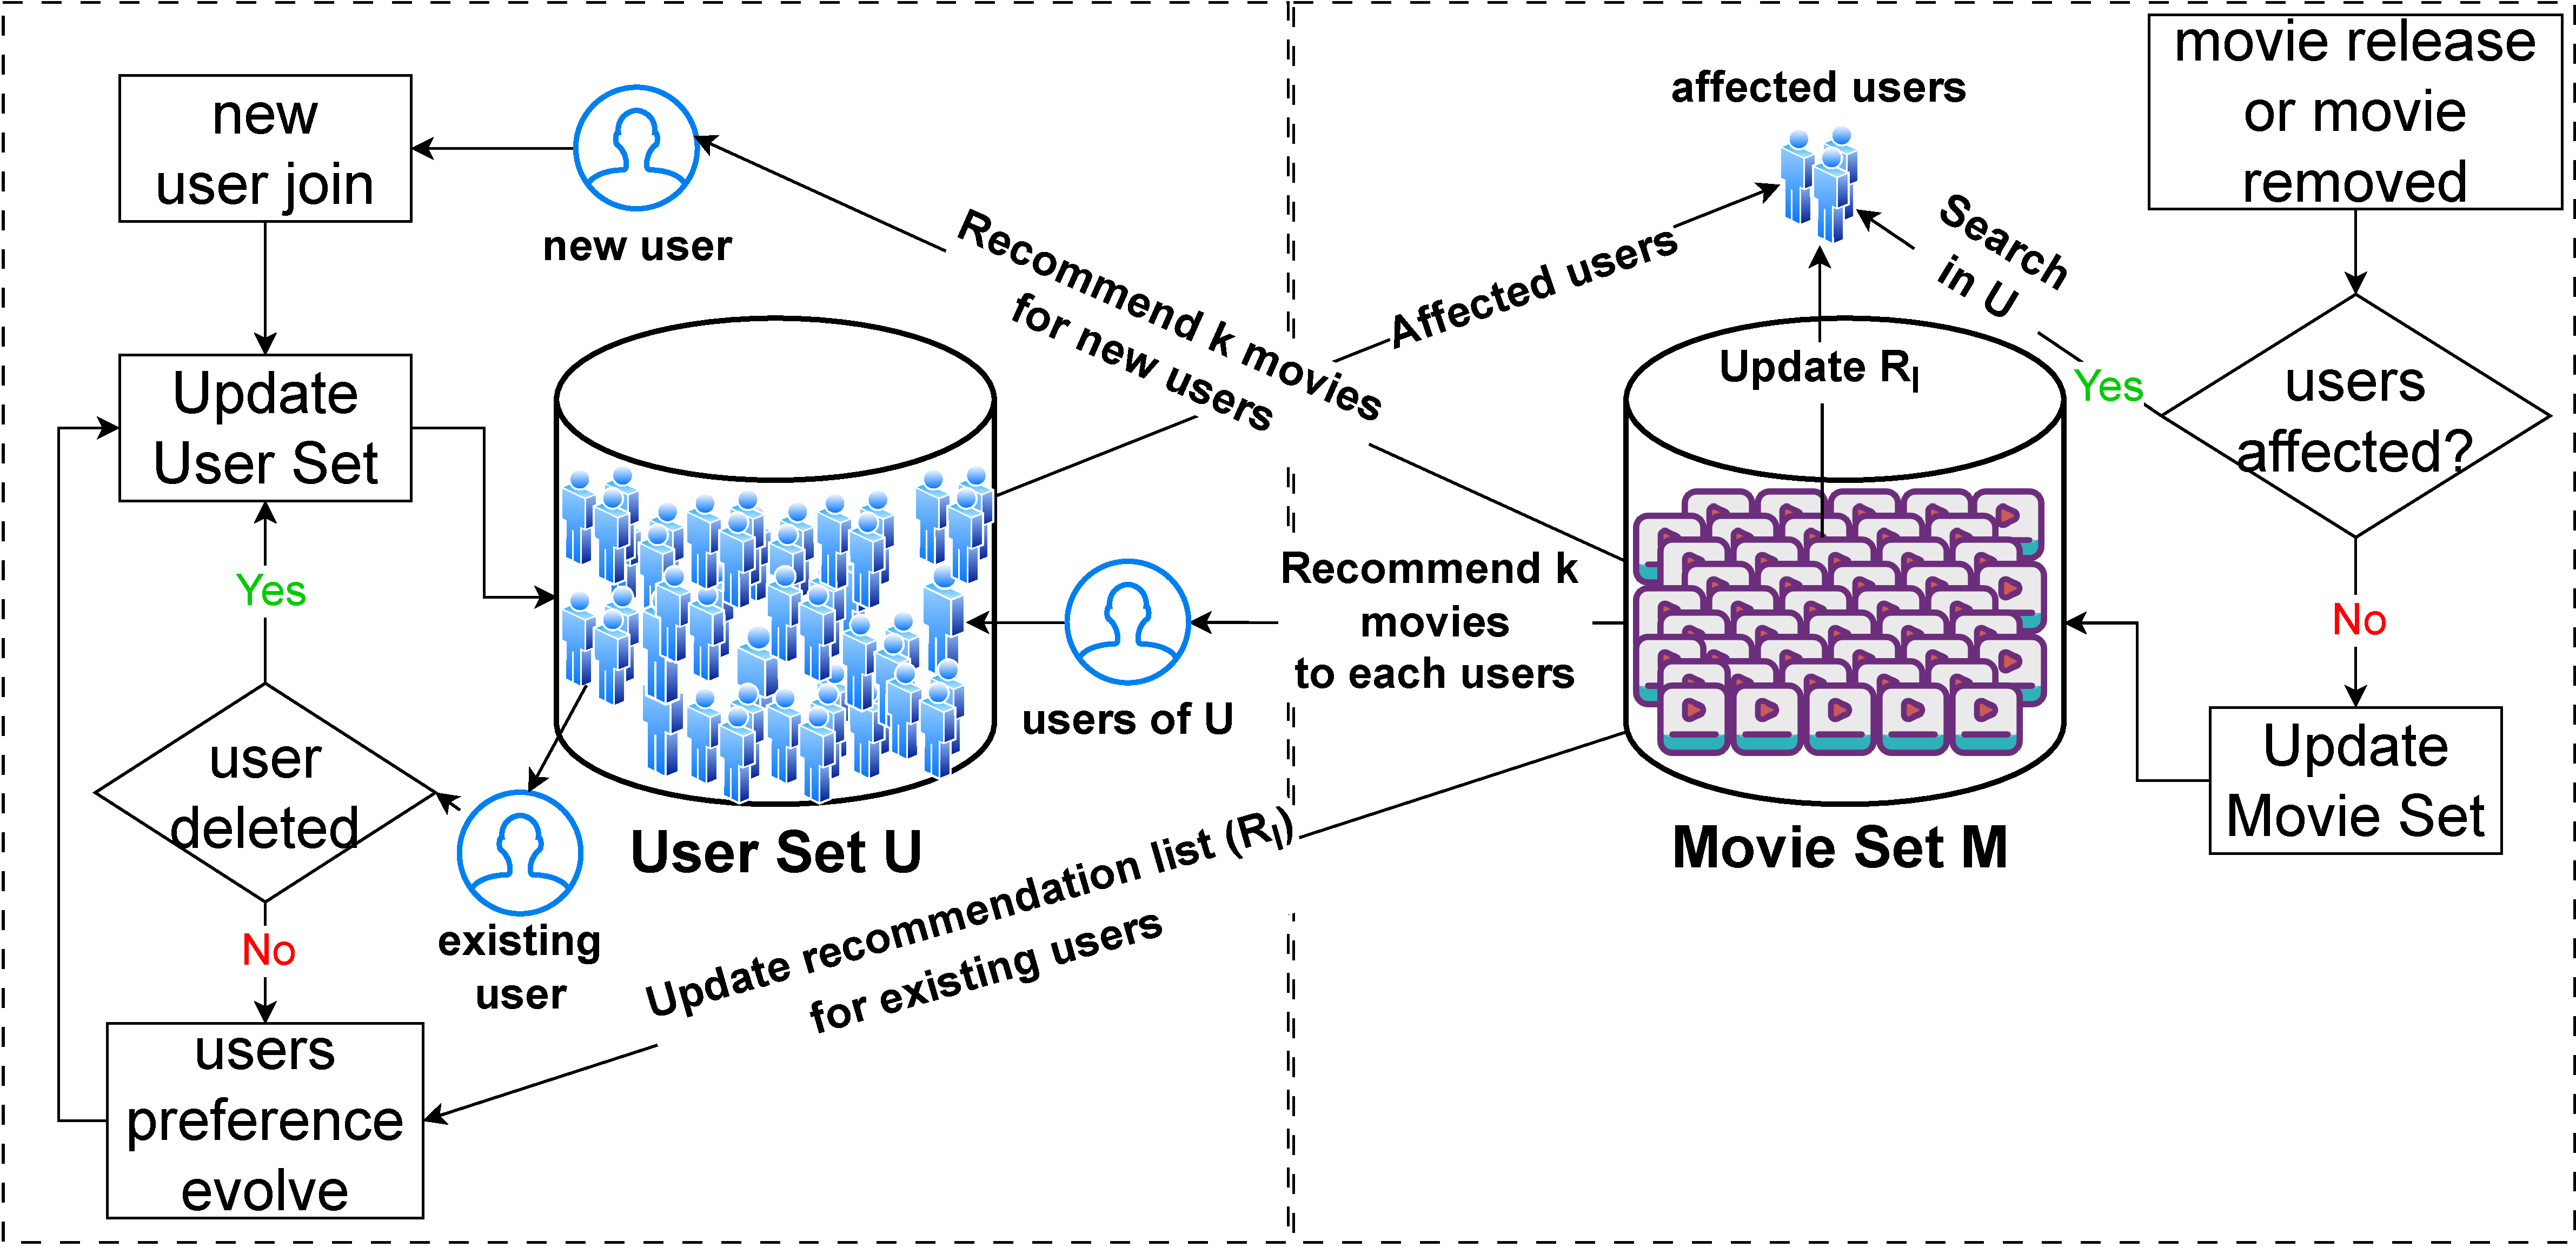
\includegraphics[width=0.45\textwidth]{Images/Movie Recommendation.pdf}
    \caption{Example of Fully Dynamic kNN Join in Movie Recommendation}
    \label{fig:recom-sys}
\end{figure}

\sstitle{1) Movie Recommendation.}
kNN join is crucial in recommendation systems, especially for movie and video streaming services, where queries (e.g., users) and answers (e.g., movies) are represented as high-dimensional vectors.
%
Traditional approaches compute the $k$ closest neighbors for each query individually, which can be computationally expensive. Employing a kNN join to compute these recommendations significantly accelerates the process~\cite{ahuja2019movie,hu2021efficient}.
%
Figure~\ref{fig:recom-sys} illustrates a \fdknnj-based recommendation system with query dataset (i.e., users $U$) and answer dataset (i.e., movies $M$). Initially, each user is recommended a set of $k$ movies from $M$. \fdknnj ensures real-time updates, adapting recommendations for new users, changing preferences, and updates in the movie dataset.
%
This scenario emphasises the capability of \fdknnj in recommendation systems, addressing new user arrivals, departures, and the dynamic nature of the content.

\sstitle{2) E-commerce.}
E-commerce sites can leverage \fdknnj to enhance product recommendations by considering the latest user interactions and purchases, increasing conversion rates and customer satisfaction.
%
In online fashion retail, user clothing preferences~\cite{liu2018clothing} evolve with seasons and fashion trends. New products are added to the inventory, while others may be discontinued or go out of stock. Additionally, new users continuously register and provide their fashion preferences.
%
The \fdknnj algorithm adeptly accommodates these changes. It seamlessly integrates new users into the user dataset, ensuring that product recommendations remain personalised and up-to-date for all users~\cite{chakraborty2021fashion}.

\sstitle{3) Healthcare and Biomedical Research.}
In the field of healthcare and biomedical research~\cite{deekshatulu2013classification,khateeb2017efficient,tayeb2017toward, bhatti2021predictive}, \fdknnj approach is valuable for understanding complex genetic information in genomics and personalised medicine. Let's consider a patient with a unique genetic profile that suggests they might be prone to a certain disease. \fdknnj can analyse their genes and compare them with similar cases to identify the best treatment options. This method is also great for keeping up with new gene therapies, as it quickly figures out which patients could benefit from the latest treatments. This method is also beneficial for keeping up with new gene therapies, as it quickly determines which patients could benefit from the latest treatments. Additionally, selecting the right medication for a patient can be facilitated by comparing their genes to their medication history. This reduces the risk of adverse reactions and ensures that the treatment is effective for the patient.

\sstitle{4) Machine Leaning.} %machine leaning
kNN join is pivotal in many machine learning applications, including classification \cite{deng2016efficient, bijalwan2014knn}, clustering \cite{yang2016fault, shi2018adaptive}, regression \cite{kohli2020sales}, predictive systems \cite{jawthari2021predicting, baashar2021predicting} and anomaly detection \cite{li2007network, tian2014anomaly, wang2020log}. Its simplicity and effectiveness in recognizing similar data points are fundamental, especially in dynamic, large-scale, high-dimensional datasets prevalent in fields like network logs and financial transactions. \fdknnj are essential for efficient dataset updates, ensuring adaptability and relevance in machine learning models.


% \sstitle{5) Supply Chain Management.}
% %
% In supply chain management, \fdknnj identifies similar suppliers for new products by comparing specifications with historical supplier data. Supply chain managers assess these suppliers based on past performance metrics. Recommendations are updated when adding new products or suppliers, and adjustments are made for products that are out of stock or no longer required.

% In supply chain management, kNN join is useful for identifying similar suppliers (Item set) for new products (User set). By comparing key specifications and requirements, such as size and materials, of new items with historical supplier data, the system identifies $k$ similar suppliers. Supply chain managers can assess these suppliers based on their past performance metrics like delivery times and product quality. Whenever a new product is added based on the demand of suppliers' requirements, then the $k$ nearest suppliers need to be recommended. Similarly, in the case of removal, if the product is out of stock or no longer required, then we need to update the dataset. 

%In supply chain management, identifying similar suppliers for new products is a critical aspect. In inventory management, the product specifications and requirements are recorded whenever a new product is added to the inventory (dataset). The key features of the new products may include things like size, weight, materials, manufacturing requirements, etc. To improve the performance of the supply chain management process, we need to perform a kNN join on the supplier dataset using the item dataset. By comparing the high-dimensional features of the new product with historical supplier data, the system identifies $k$ suppliers whose products or services are most similar to the new products. Similarity metrics, such as Euclidean distance or cosine similarity, can be used to measure the similarity between the new product and existing supplier offerings.

%With the help of the kNN join approach, the supply chain manager will get a list of $k$ similar suppliers. The supply chain manager can then assess these suppliers' historical performance metrics, such as delivery timelines, product quality, and customer satisfaction scores, to decide which supplier to choose for the new product.
%When there are changes in market demand or customer preferences, the demand patterns for certain products in the inventory might shift. Accordingly, we need to update the item dataset.

%The inventory management system can recommend strategies used for similar products in the past. If a similar product faced supply chain disruptions or had successful inventory clearance strategies, the supply chain manager could apply similar tactics to the current product. By learning from historical data on similar products, the system assists in optimising inventory levels, reducing excess stock, ensuring products are available when needed, and eliminating suppliers who are not trustworthy or reliable. In this dynamic scenario, the kNN join operation needs to be recalculated whenever a new product is added, demand patterns change or supplier performance metrics are updated.

\sstitle{5) LLMs and Vector Databases.}
The fusion of large language models (LLMs) \cite{kassner2020bert, song2023llm, kasneci2023chatgpt}, vector databases \cite{stata2000term, okorie2011nigeria, singla2021experimental, han2023comprehensive, pan2023survey}, and \fdknnj brings benefits for question-answering systems or personalised news subscriptions.
%
Users express interests in natural language, and LLMs convert them into high-dimensional vectors. These vectors are used for kNN queries on the dynamic content dataset, with \fdknnj ensuring real-time updates for database and user query changes. This applies to new query registrations or removals, addition of new content, and removal of expired content.% from the vector database.
\end{comment}

\noindent \textbf{CONTRIBUTIONS.} We present \dualtree, a symmetric dual-index framework for high-dimensional kNN joins that supports interleaved updates on both datasets, enabling efficient high-dimen\-sional kNN join in fully-dynamic scenarios. In parallel, we introduce a point-wise, fine-grained pruning mechanism driven by a cost-aware model that quantitatively bridges projection dimensionalities to computation cost, yielding the theoretically optimal pruning dimensionality and driving pruning efficiency toward its maximal limit.
%
Our key contributions are as follows:

\begin{comment}
\begin{enumerate} [leftmargin=*, wide, labelindent=0pt]
    \item \underline{\emph{\fdknnj with Dual-index Schema.}}
    We introduce a novel approach explicitly designed for \fdknnj over high-dimensional data. Unlike existing dynamic methodologies \cite{yu2010high, yang2014continuous, ukey2022efficient, ukey2023efficient} where updates primarily focus on the answer set, our method adeptly manages updates on both query and answer sets.
    %
    We introduce a \emph{dual-index} schema, building separate index structures for the query and answer datasets. Specifically, we utilise the \hdrtree \cite{yang2014continuous} for the query set and the \deltatree \cite{cui2003contorting} for the answer set. While the original \hdrtree lacks support of updating, we design an algorithm for efficient dual-index maintenance in \fdknnj.
    %
    To the best of our knowledge, this is the first work to study the problem of \fdknnj over high-dimensional data.
    %
    Furthermore, we also propose an effective cluster-based optimise to further accelerate batch updates.

    \item \underline{\emph{Cost-oriented Fine-gained Pruning.}}
    %
    We introduce a fine-grained \emph{item-level} pruning technique, which includes an additional pruning step in a lower dimension within the leaf nodes of the index tree to further remove unpromising data points for the current update.
    %
    Our approach is lightweight and seamlessly integrates with existing index structures, including the \hdrtree and \deltatree used in our dual-index schema.
    %
    To determine the optimal dimensionality for our fine-grained pruning, we derive a cost function to estimate the cost of updates when applying different dimensionalities in the pruning strategy. By employing sampling to estimate the parameters in the cost function, our method can decide the optimal dimensionality for the fine-grained pruning.
    % sample
    % support single/batch update
    

    \item \underline{\emph{Extensive Experiments on Real-World Datasets.}}
    \todo{}
    We conducted an extensive experimental analysis to evaluate the performance of our novel, \fdknnj approach. To assess its effectiveness, we compared it with the existing partially dynamic kNNJoin$^+$ approach. These experiments are conducted using a range of real-world datasets with varying dimensionalities. Our work marks a significant contribution to the field as it introduces a fully dynamic approach, and our results prove that our approach is scalable and efficient as compared to existing solutions.
    
\end{enumerate}
\end{comment}

\noindent(1)\underline{\emph{\fdknnj with Dual-index Schema.}}
   We introduce \dualtree, a symmetric dual-indexing framework that leverages an \hdrtree on the query set for reverse kNN (RkNN) searches and a \deltatree on the reference set for forward kNN searches. Crucially, both index structures support incremental updates according to the updates of their corresponding sets. This dual capability allows \dualtree to maintain the kNN join table with low when both datasets evolve concurrently.


\noindent(2)\underline{\emph{Cost-oriented Fine-gained Pruning.}}
    We augment \dualtree with a point-wise low-dimensional pruning stage that filters, at low cost, a large fraction of false positives that survive prior cluster-level pruning. Unlike existing kNN join systems, we characterize the distributional behavior of interpoint distances and develop an approximate relation between the projection dimensionalities and projected distances. Building on this, we formulate a cost-aware model that links the pruning dimensionalities to computational expense, based on which, we derive the optimal projection dimensionality and drives pruning efficiency toward its theoretical maximum. To our knowledge, this is the first quantitative treatment that couples pruning dimensionalities with computational cost in kNN join.
    

\noindent(3)\underline{\emph{Extensive Experiments on Real-World Datasets.}}
   We evaluate on 8 real-world datasets spanning wide dimensionalities (128d to 4096d). As baselines, we select the strongest publicly available kNN join methods that can still be applied to fully-dynamic and high-dimen\-sional workloads, albeit not specialized for this regime. Across all datasets, our dual-index framework achieves clearly higher speed. Furthermore, experiment results demonstrate that, the point-wise, cost-aware pruning strategy provides an additional, substantial performance boost to the \dualtree framework.
    



\begin{comment}
\stitle{Outline.} 
%
The remaining paper is organised as follows. Section \ref{sec:background} introduces problem definitions and preliminaries. Section \ref{sec:related-works} reviews related literature. Section \ref{sec:fdknnj} and Section \ref{sec:pruning} present our proposed dual-index schema and cost-oriented fine-grained pruning, respectively. Section \ref{sec:exp} presents the experimental results, followed by the conclusion in Section \ref{sec:conclusion}.
\end{comment}